\documentclass{report}

\usepackage[utf8]{inputenc}
\usepackage[top=1cm, bottom=2cm, left=2cm, right=2cm]{geometry}
\usepackage[francais]{babel}
\usepackage[T1]{fontenc}
\usepackage{graphicx}
\usepackage{subcaption}
\usepackage{listings}
\usepackage{hyperref}
\usepackage{wrapfig}
\usepackage{lmodern}

\title{Rapport}
\author{François PIAT}
\date{WEEK 9}

\begin{document}
\maketitle

\chapter*{Profiling}
\paragraph{Vérification résultats "Transform-image"}
Afin de vérifier les bons résultats obtenus en semaine 5 pour transform-image, j'ai réalisé les test de profiling à nouveau sur l'interpolation gaussienne de Transform-image. \\
\textit{Le taux obtenu est de x6.48, contre x7.39 la première fois};





\chapter*{Implémentation}	

\paragraph{Stratégie}
- On a continué la programmation des différentes options de BOOST pour pouvoir avancer plus loin et maintenant implémenter des utilisations de back-ends automatiquement détectés.\\
- Il a fallu créer un projet "MyTransform" afin de ré-implémenter la fonction "transform-image".\\
- En fin de semaine, il a été convenu de repartir de 0 pour les fonctions déjà étudiées (smooth-image et transform-image), en utilisant de préférence un langage plus récent et plus adapté que le C++. \\
La décision a été orientée par Ghislain (mon tuteur), me laissant le choix tout de même entre le langage RUST et PYTHON. Ainsi, j'ai dû réaliser un petit programme utilisant quelques fonctions de déclarations de tableaux avec l'API d'arrayfire dans les 2 langages différents : Python et Rust. Mes conclusions sont dans le paragraphe "Résultats". 

\paragraph{Problèmes}
- Problème de bibliothèque avec python (et tuteur absent) => pas de programme prêt à temps.

\paragraph{Résultats}
- Suite a la programmation/discussion autour de Rust et Python, on peut relever les points forts suivants : 
\begin{figure}[h!]
	\begin{center}
		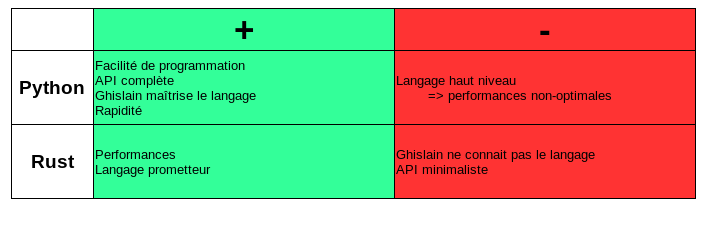
\includegraphics[width=19cm]{figures/tableau_comparatigf.png}
	\end{center}	
	\caption{Comparaison de Rust et Python pour MIRTK}
	\label{Comparaison de Rust et Python pour MIRTK}
\end{figure}

- Il faut aussi ajouter à cela le fait que je ne connais pas réellement de langage de haut-niveau (excepté MATLAB), et ça serait l'occasion d'apprendre le langage PYTHON.\\

- Après avoir codé quelques lignes en RUST avec Arrayfire, je peux de même affirmer que le wrap en RUST d'ArrayFire est minimaliste: la liste des fonctions disponibles n'est pas exhaustive, les fonctions ont souvent une seule signature possible, peu de templates...\\
\\
\\
Pour cette raison, je pense m'intéresser au PYTHON plutôt qu'au RUST pour ce projet.
\end{document}